% Gemini theme
% See: https://rev.cs.uchicago.edu/k4rtik/gemini-uccs
% A fork of https://github.com/anishathalye/gemini

\documentclass[final]{beamer}

% ====================
% Packages
% ====================
\usepackage{amsfonts}
\usepackage[T1]{fontenc}
\usepackage{lmodern}
\usepackage[size=custom,width=120,height=72,scale=1.0]{beamerposter}
\geometry{paperwidth=48in,paperheight=36in}
\usetheme{gemini}
\usecolortheme{ucf}
\usepackage{graphicx}
\usepackage{booktabs}
\usepackage{tikz}
\usepackage{pgfplots}
\pgfplotsset{compat=1.14}

\usepackage{float}
\usepackage{xspace}
\usepackage{graphicx}
\graphicspath{{./imgs/}}
\usepackage{comment}
\usepackage{listings,hyperref}
\usepackage{cite}

% nice looking audit titles
\newcommand{\Minerva}{\textsc{Minerva}\xspace}
\newcommand{\Prov}{\textsc{Providence}\xspace}
\newcommand{\B}{{{B2}}\xspace}
\newcommand{\R}{{{R2}}\xspace}
\newcommand{\BRAVO}{\textsc{BRAVO}\xspace}


% ====================
% Lengths
% ====================

% If you have N columns, choose \sepwidth and \colwidth such that
% (N+1)*\sepwidth + N*\colwidth = \paperwidth
\newlength{\sepwidth}
\newlength{\colwidth}
\setlength{\sepwidth}{0.001\paperwidth}
\setlength{\colwidth}{0.23\paperwidth}

\newcommand{\separatorcolumn}{\begin{column}{\sepwidth}\end{column}}

% ====================
% Title
% ====================

\title{Election Security with Risk-Limiting Audits}

%\author{Nitish A. Gupta \inst{1} \and Nitish A. Gupta \inst{2}}
\author{Oliver Broadrick\inst{1} \and
Poorvi L. Vora\inst{1} \and
Filip Zag{\'o}rski\inst{2}\inst{3}}
% First names are abbreviated in the running head.
% If there are more than two authors, 'et al.' is used.
%
\institute[shortinst]{\inst{1} Department of Computer Science, The George Washington University%\thanks{Supported in part by NSF Award 2015253} 
\samelineand \inst{2} Wroclaw University of Science and Technology%\thanks{Author was partially supported by Polish National Science Centre contract number DEC-2013/09/D/ST6/03927} and 
\samelineand \inst{3} Votifica
}
%

%\institute[shortinst]{\inst{1} \textit{University of Central Florida, Orlando, FL} \samelineand \inst{2} Another Institute}

% ====================
% Footer (optional)
% ====================

\footercontent{
  \href{odbroadrick@gmail.com}{odbroadrick@gmail.com}
}
% (can be left out to remove footer)

% ====================
% Logo (optional)
% ====================

% use this to include logos on the left and/or right side of the header:
% \logoright{\includegraphics[height=7cm]{logo1.pdf}}
% \logoleft{\includegraphics[height=7cm]{logo2.pdf}}

% ====================
% Body
% ====================

\begin{document}
\addtobeamertemplate{headline}{}
{
    \begin{tikzpicture}[remember picture,overlay]
      \node [anchor=north west, inner sep=3cm] at ([xshift=0.0cm,yshift=3cm]current page.north west)
      {
\includegraphics[height=8cm]{logos/gw.png}}; % also try shield-white.eps
      \node [anchor=north east, inner sep=3cm] at ([xshift=0.0cm,yshift=3cm]current page.north east)
      {
\includegraphics[height=8cm]{logos/gw.png}};
    \end{tikzpicture}
}

\begin{frame}[t]
\begin{columns}[t]
\separatorcolumn

\begin{column}{\colwidth}

\begin{block}{Original Contributions}

Risk-Limiting Audits (RLAs) are rigorous election audits performed in rounds. 
Most commonly used RLAs EoR \BRAVO and SO \BRAVO (Stark) rely on the Sequential Probability Ratio Test (SPRT), using
a ratio of sample probabilities conditioned on alternative and null hypotheses.
Newer RLA \Minerva (Vora) uses a ratio of the tails of those distributions, requiring half as many
ballots as EoR \BRAVO in the first round when probability of stopping is $0.9$.
\Minerva was used in a pilot RLA in Montgomery County, Ohio in 2020,
and is recommended by the largest US voting organizations: Verified Voting, the Brennan Center, and Common Cause, 
It is unknown how the audits compare in later rounds or with lower stopping probabilities, a problem with no easy analytical approach.
Unlike EoR and SO \BRAVO, \Minerva is proven to be risk-limiting only when round sizes are predetermined, 
meaning round sizes cannot be chosen based on previous samples.
\begin{itemize}
\item
We provide simulations of EoR \BRAVO, SO \BRAVO, and \Minerva that help us understand their behavior across multiple rounds and with lower
first round stopping probability; this information can be used to advise election officials.
\item
We introduce \Prov, an RLA which has the efficient tail ratio approach of \Minerva but is resistant to an adversary who can pick
future round sizes with knowledge of previous samples. \Prov was named after the Rhode Island city where it was used for a public
pilot audit in February 2022.
\end{itemize}
\end{block}

\begin{block}{Results}

\begin{itemize}
\item Both \BRAVO audits are more conservative than \Minerva, which stops with fewer ballots, for both first round stopping probabilities. 
However, the advantage of using \Minerva decreases considerably for the smaller first round stopping probability.
\item Proofs that \Prov is risk-limiting and resistant to an adversary who can pick future round sizes with knowledge of previous samples.
\end{itemize}
\end{block}

\begin{block}{Risk-Limiting Audits}

\begin{itemize}
\item
A risk-limiting audit (RLA) draws paper ballots in rounds, stopping if a rigorous statistical criterion is satisfied, or proceeding to a full hand count. If the announced outcome of the election is erroneous, an RLA will detect the error with high, predetermined minimum probability. 
\item
An audit $\mathcal{A}$ takes a sample of ballots $X$ as input and gives as output either
(1) $Correct$: the audit is complete, or (2) $Uncertain$: continue the audit.
\item
The maximum risk $R$ of audit $\mathcal{A}$ with sample $X\in \{0,1\}^*$ drawn from 
the true underlying distribution of ballots is
$$R(\mathcal{A})=\Pr[\mathcal{A}(X)=Correct \mid H_0],$$ where $H_0$ is the null
hypothesis: the true underlying election is a tie.
\item
An audit $\mathcal{A}$ is a Risk-Limiting Audit with 
risk limit $\alpha$ iff 
$$R(\mathcal{A}) \le \alpha.$$
\end{itemize}
\end{block}

\begin{block}{Simulations}

\begin{itemize}
\item 
Software: R2B2 library\cite{r2b2} which has Python implementations of several RLAs as well as a simulator
\item 
Risk limit: 10\%
\item
Margins: 2020 US Presidential election statewide results, limiting ourselves to pairwise margins
for the two main candidates of $0.05$ or larger
\item 
Trials per state: $10,000=10^4$ audits assuming the underlying election is as announced,  
and $10,000=10^4$ audits assuming the underlying election is a tie
\item 
Round schedules: EoR \BRAVO and SO \BRAVO round sizes are chosen to achieve the same
probability of stopping in each round given preceding samples. \Minerva first round sizes
are chosen to achieve some probability of stopping and subsequent round sizes are given by multiplying the previous
round size by $1.5$ or by $1.0$.
\end{itemize}
\end{block}

\end{column}

\separatorcolumn

\begin{column}{\colwidth}

\begin{block}{Risk}

\begin{itemize}
\item 
All audits have estimated risks below the risk limit
\item
EoR \BRAVO falls an order of magnitude less than the others, unnecessarily conservative
\end{itemize}

\begin{figure}[h]
\centering
\begin{minipage}{.49\textwidth}
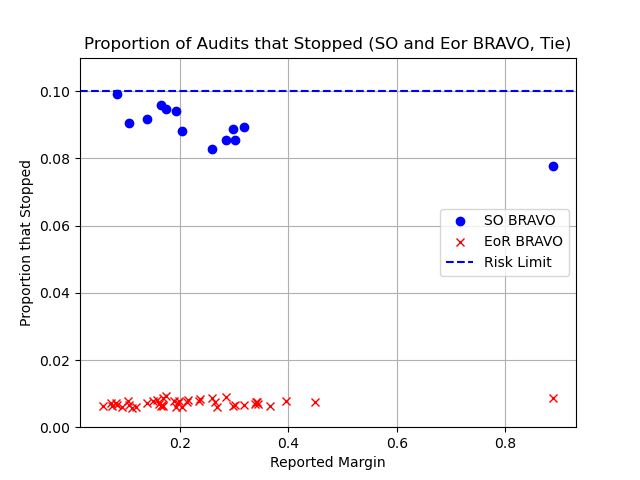
\includegraphics[width=\textwidth]{bravo_risks.png}
\label{fig:bravo_risk}
\end{minipage}
\begin{minipage}{.49\textwidth}
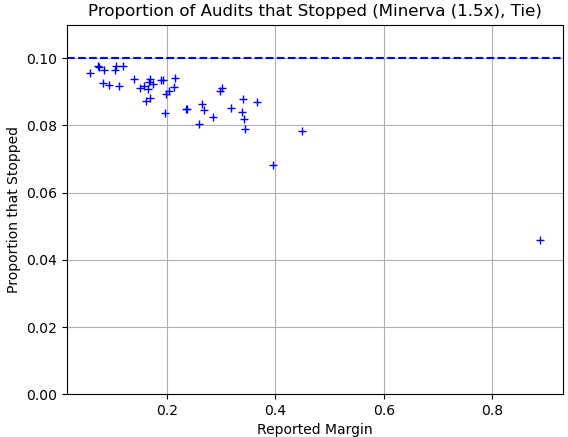
\includegraphics[width=1.0\textwidth]{riskminerva1p5_10t4.png}
\label{fig:minerva_risk}
\end{minipage}
\caption{These plots show for $\chi_1=0.9$ the fraction of audits (EoR \BRAVO (left), SO \BRAVO (left), and \Minerva with multiplier $1.5$ (right)) that stopped in any of the $5$ rounds when the underlying election was a tie. (For SO \BRAVO audits we show the 13 states for which simulations are complete.)}
%\label{fig:risk}
\end{figure}

\end{block}


\begin{block}{Stopping Probability}

\begin{itemize}
\item
Conditional stopping probability, $\chi_j$, is the probability that an audit will stop in round $j$ given that it did not stop earlier, and in 
simulations $\chi_j$ is estimated by the proportion of audits that stop in a round to those that ``entered'' that round
i.e. those that did not stop before round $j$. 
%The conditional stopping probability  of an audit $\mathcal{A}$ in round $j$ is 
%$$\chi_j (\mathcal{A})=\Pr[\mathcal{A}(X)=Correct ~in~round~j~\mid H_a \land \mathcal{A}(X) \neq Correct ~previously]$$
\end{itemize}

\begin{figure}[h]
\centering
\begin{minipage}{.49\textwidth}
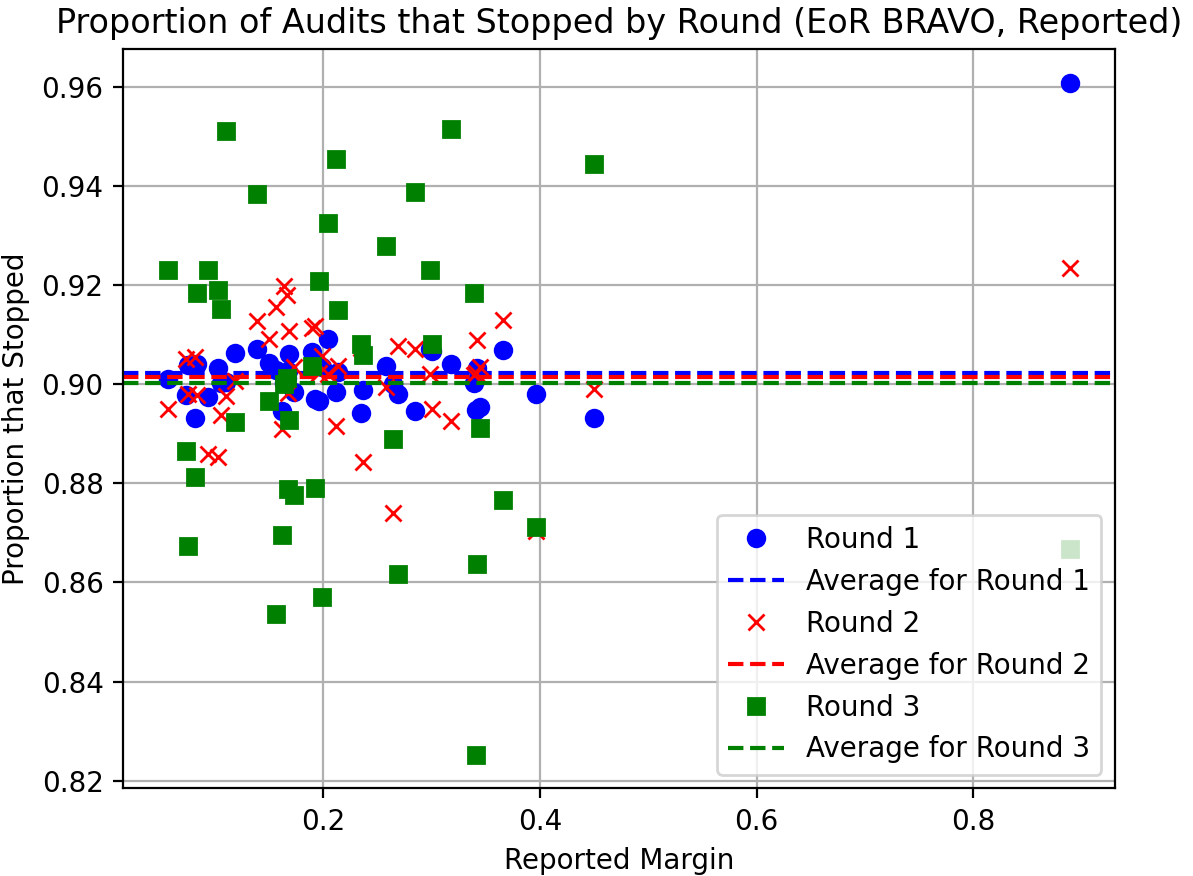
\includegraphics[width=1.0\textwidth]{eor_bravo_90perc_10^4_corrected/sprob_first_three_cropped.png}
\label{fig:eor_bravo_sprob}
\end{minipage}
\begin{minipage}{.49\textwidth}
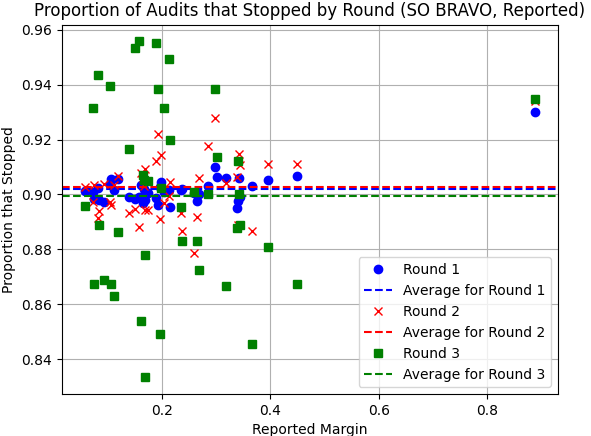
\includegraphics[width=1.0\textwidth]{so_bravo_90perc_10^4/sprob_first_three.png}
\label{fig:so_bravo_sprob}
\end{minipage}
\caption{These plots show, for each state margin, when the underlying election is as announced, the number of audits that stopped in the $j^{th}$ round, as a fraction of all audits which had not yet stopped before the $j^{th}$ round for $j=1,2,3$ and $\chi_j=0.9$. The left shows EoR \BRAVO and the right shows SO \BRAVO.}
\end{figure}

\begin{figure}[h]
\centering
\begin{minipage}{.49\textwidth}
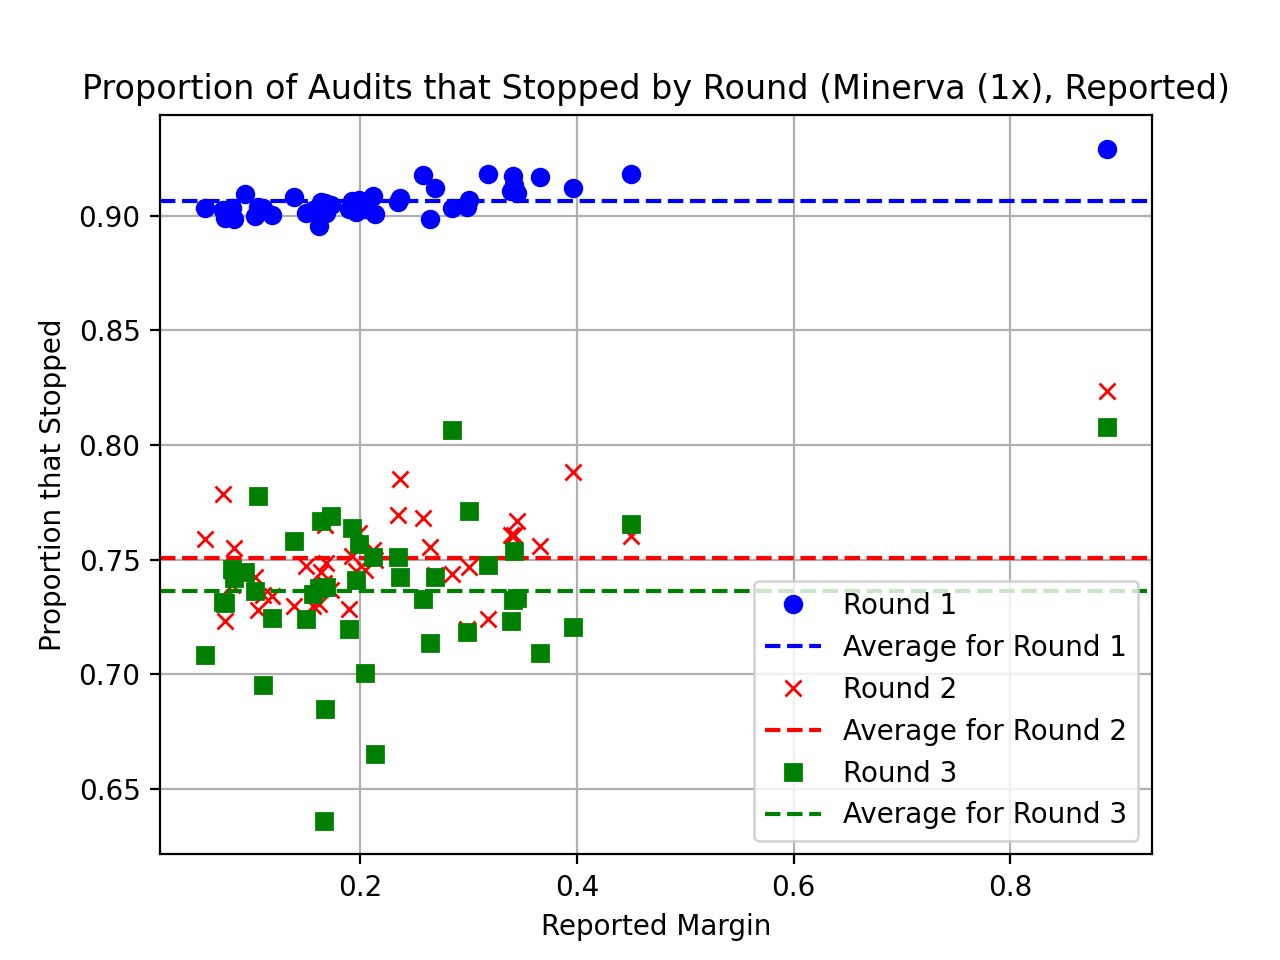
\includegraphics[width=1\textwidth]{minerva_multiround_1x_10^4/sprobs_first_three.png}
\label{fig:minerva1_sprob}
\end{minipage}
\begin{minipage}{.49\textwidth}
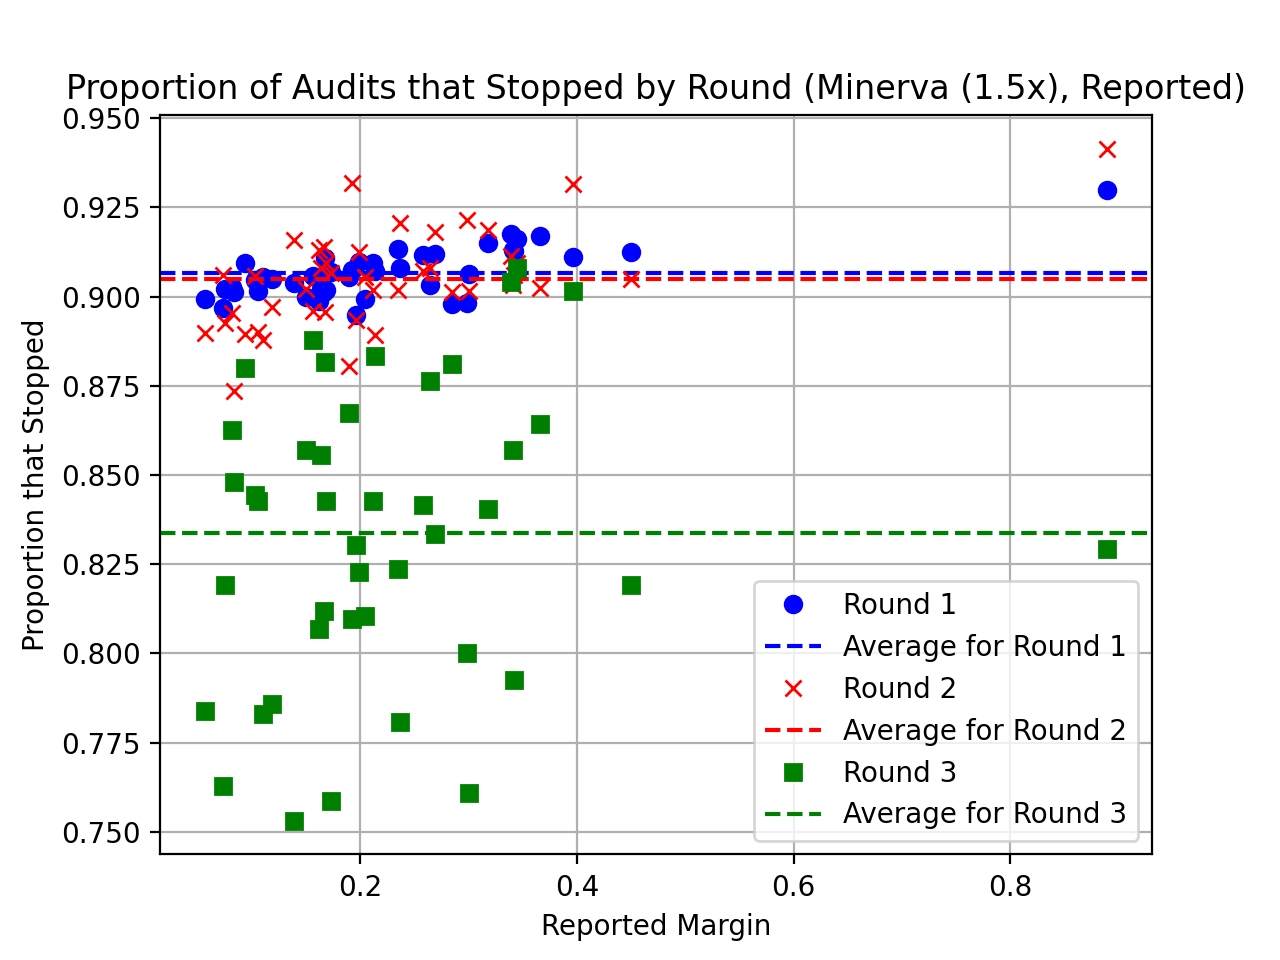
\includegraphics[width=1\textwidth]{minerva_multiround_1p5x_10^4/sprobs_first_three.png}
\label{fig:minerva1p5_sprob}
\end{minipage}
\caption{These plots show, for each state margin, when the underlying election is as announced, the number of \Minerva audits that stopped in the $j^{th}$ round, as a fraction of all \Minerva audits which had not yet stopped before the $j^{th}$ round for $j=1,2,3$. The left shows \Minerva with the round schedule obtained by $\chi_1=0.9$ and round size multiple $1.5$.}
\end{figure}

We also consider a first round size with $\chi_1=0.25$. 

\begin{figure}
\begin{centering}
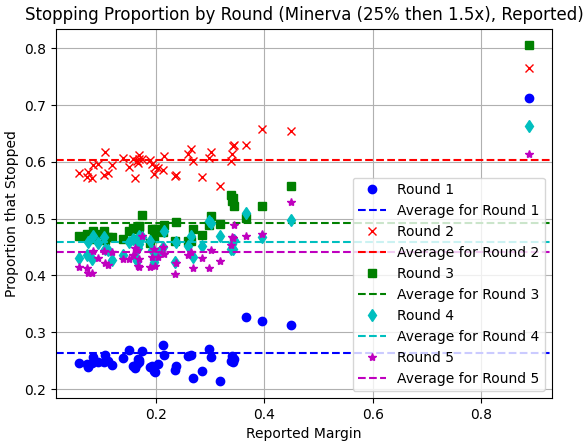
\includegraphics[width=0.6\textwidth]{minerva25percthen1p5_sprob.png}
\caption{This plot shows, for each state margin, when the underlying election is as announced, the number of \Minerva audits that stopped in the $j^{th}$ round,
as a fraction of all \Minerva audits which had not yet stopped before the $j^{th}$ round for $j=1,2,3$, round size multiple of $1.5$ and $\chi_1 = 0.25$.}
\label{fig:minerva_25}
\end{centering}
\end{figure}

  \end{block}

%  \begin{block}{Fusce aliquam magna velit}
%
%    Et rutrum ex euismod vel. Pellentesque ultricies, velit in fermentum
%    vestibulum, lectus nisi pretium nibh, sit amet aliquam lectus augue vel
%    velit. Suspendisse rhoncus massa porttitor augue feugiat molestie. Sed
%    molestie ut orci nec malesuada. Sed ultricies feugiat est fringilla
%    posuere.
%
%    \begin{figure}
%      \centering
%      \begin{tikzpicture}
%        \begin{axis}[
%            scale only axis,
%            no markers,
%            domain=0:2*pi,
%            samples=100,
%            axis lines=center,
%            axis line style={-},
%            ticks=none]
%          \addplot[red] {sin(deg(x))};
%          \addplot[blue] {cos(deg(x))};
%        \end{axis}
%      \end{tikzpicture}
%      \caption{Another figure caption.}
%    \end{figure}
%
%  \end{block}
%
%  \begin{block}{Nam cursus consequat egestas}
%
%    Nulla eget sem quam. Ut aliquam volutpat nisi vestibulum convallis. Nunc a
%    lectus et eros facilisis hendrerit eu non urna. Interdum et malesuada fames
%    ac ante \textit{ipsum primis} in faucibus. Etiam sit amet velit eget sem
%    euismod tristique. Praesent enim erat, porta vel mattis sed, pharetra sed
%    ipsum. Morbi commodo condimentum massa, \textit{tempus venenatis} massa
%    hendrerit quis. Maecenas sed porta est. Praesent mollis interdum lectus,
%    sit amet sollicitudin risus tincidunt non.
%
%    Etiam sit amet tempus lorem, aliquet condimentum velit. Donec et nibh
%    consequat, sagittis ex eget, dictum orci. Etiam quis semper ante. Ut eu
%    mauris purus. Proin nec consectetur ligula. Mauris pretium molestie
%    ullamcorper. Integer nisi neque, aliquet et odio non, sagittis porta justo.
%
%    \begin{itemize}
%      \item \textbf{Sed consequat} id ante vel efficitur. Praesent congue massa
%        sed est scelerisque, elementum mollis augue iaculis.
%        \begin{itemize}
%          \item In sed est finibus, vulputate
%            nunc gravida, pulvinar lorem. In maximus nunc dolor, sed auctor eros
%            porttitor quis.
%          \item Fusce ornare dignissim nisi. Nam sit amet risus vel lacus
%            tempor tincidunt eu a arcu.
%          \item Donec rhoncus vestibulum erat, quis aliquam leo
%            gravida egestas.
%        \end{itemize}
%      \item \textbf{Sed luctus, elit sit amet} dictum maximus, diam dolor
%        faucibus purus, sed lobortis justo erat id turpis.
%      \item \textbf{Pellentesque facilisis dolor in leo} bibendum congue.
%        Maecenas congue finibus justo, vitae eleifend urna facilisis at.
%    \end{itemize}
%    
%    Nulla eget sem quam. Ut aliquam volutpat nisi vestibulum convallis. Nunc a
%    lectus et eros facilisis hendrerit eu non urna. Interdum et malesuada fames
%    ac ante \textit{ipsum primis} in faucibus. Etiam sit amet velit eget sem
%    euismod tristique. Praesent enim erat, porta vel mattis sed, pharetra sed
%    ipsum. Morbi commodo condimentum massa, \textit{tempus venenatis} massa
%    hendrerit quis. Maecenas sed porta est. Praesent mollis interdum lectus,
%    sit amet sollicitudin risus tincidunt non.
%  \end{block}
%
\end{column}

\separatorcolumn

\begin{column}{\colwidth}


\begin{block}{Number of Ballots}
\begin{itemize}
\item
The number of ballots sampled is one crude measure of the workload of an audit.
To keep the costs of RLAs low, audits should be designed to stop with as few ballots as possible.
\item
The following plots show the probability of stopping as a function of the average number of ballots
sampled by round in our simulations.
\end{itemize}

\begin{figure}[h]
\centering
\begin{minipage}{.49\textwidth}
\begin{centering}
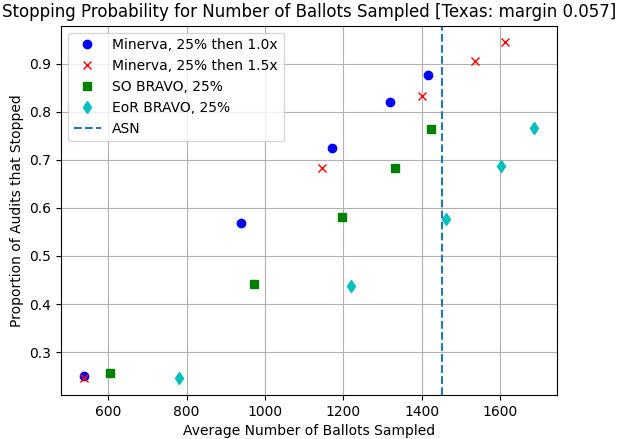
\includegraphics[width=1\textwidth]{texas25.png}
%\caption{This plot shows the cumulative fraction of audits that stopped as a function of average number of sampled ballots for all four audits we studied, for the state of Texas, margin $0.057$, and first round stopping probability $S_1=0.25$.}
\label{fig:texas_25}
\end{centering}
\end{minipage}
\begin{minipage}{.49\textwidth}
\begin{centering}
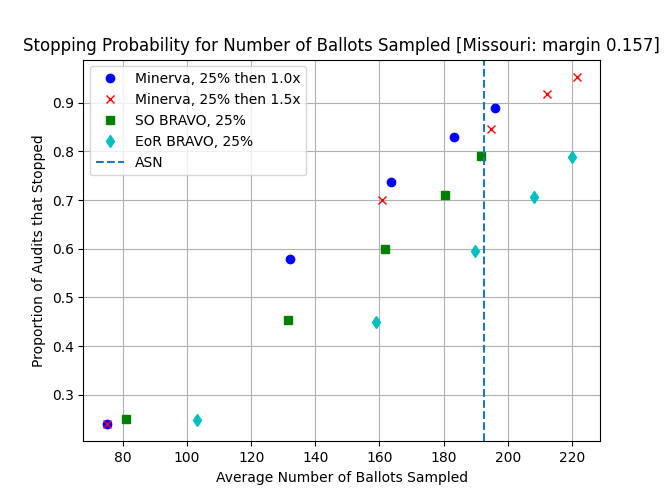
\includegraphics[width=1\textwidth]{missouri25.png}
%\caption{This plot shows the cumulative fraction of audits that stopped as a function of average number of sampled ballots for all four audits we studied, for the state of Missouri, margin $0.157$, and first round stopping probability $S_1=0.25$.}
\label{fig:missouri_25}
\end{centering}
\end{minipage}
\caption{These plots show the cumulative fraction of audits that stopped as a function of average number of sampled ballots for all four audits we studied, for the states of Texas with margin $.057$ (left) and Missouri with margin $0.157$ (right), both with first round stopping probability $\chi_1=0.25$.}
\end{figure}

\begin{figure}[h]
\centering
\begin{minipage}{.49\textwidth}
\begin{centering}
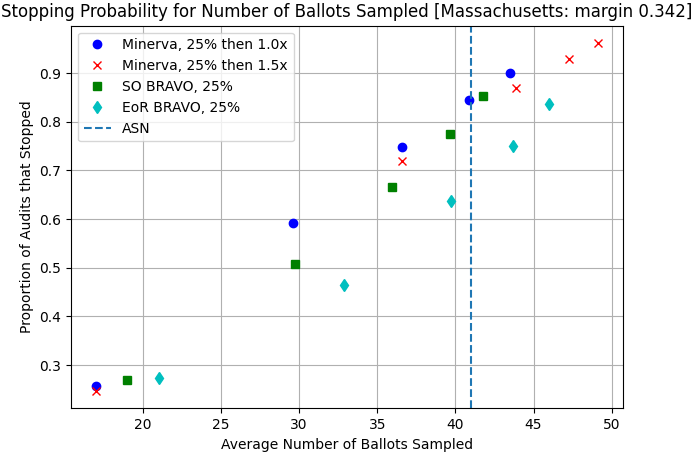
\includegraphics[width=1\textwidth]{massachusetts25.png}
%\caption{This plot shows the cumulative fraction of audits that stopped as a function of average number of sampled ballots for all four audits we studied, for the state of Massachusetts, margin $0.342$, and first round stopping probability $\chi_1=0.25$.}
\label{fig:mass_25}
\end{centering}
\end{minipage}
\begin{minipage}{.49\textwidth}
\begin{centering}
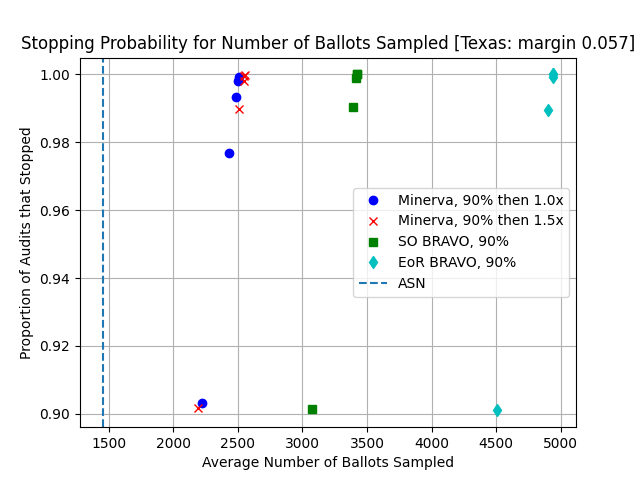
\includegraphics[width=1\textwidth]{texas90.png}
%\caption{This plot shows the cumulative fraction of audits that stopped as a function of average number of sampled ballots for all four audits we studied, for the state of Texas, margin $0.057$, and first round stopping probability $\chi_1=0.9$.}
\label{fig:texas_90}
\end{centering}
\end{minipage}
\caption{These plots show the cumulative fraction of audits that stopped as a function of average number of sampled ballots for all four audits we studied, for the states Massachusetts (left) with margin $0.342$ and $\chi_1=0.25$ and Texas (right) with margin $0.057$ and $\chi_1=0.9$.}
\end{figure}

For $\chi_1=0.25$, the ratio of first round size of EoR \BRAVO to \Minerva is $1.45$, $1.37$, $1.23$ for states Texas, Missouri and Massachusetts, and margins $0.057$, $0.157$ and $0.342$ respectively. This may be compared to $2.03$, $1.99$ and $1.8$ respectively for $\chi_1=0.9$. Similarly, for $\chi_1=0.25$, the ratio of first round size of SO \BRAVO to \Minerva is $1.13$, $1.08$, $1.12$ for states Texas, Missouri and Massachusetts, and margins $0.057$, $0.157$ and $0.342$ respectively. This may be compared to $1.38$, $1.38$ and $1.30$ respectively for $\chi_1=0.9$. 


\end{block}





%work load workload WORKLOAD
%\begin{block}{Modeling Workload}
%
%\emph{I initially wrote this section since I'd really like to have some evidence that for certain workload parameters, we see an optimal
%number of rounds greater than 1 with Providence. I am working on that code now.}
%
%\BRAVO requires the smallest expected number of ballots when ballots are drawn one at a time and the (true) underlying election is as announced. 
%In real audits, election officials draw ballots in rounds because their is some overhead with each round (e.g. opening ballot boxes).
%Therefore a more sophisticated workload model has a per ballot cost $c_b$ and a per round cost $c_r$. 
%Let $n$ be the number of ballots sampled and $j$ be the number of rounds. Then the cost $C$ is given by 
%$$C(n,j) = c_b\cdot n + c_r\cdot j,$$
%and depending on the ratio between $c_b$ and $c_r$, we should expect that certain round schedules
%achieve lower expected cost.
%\end{block}




%  \begin{block}{A block containing some math}
%
%    Nullam non est elit. In eu ornare justo. Maecenas porttitor sodales lacus,
%    ut cursus augue sodales ac.
%
%    $$
%    \int_{-\infty}^{\infty} e^{-x^2}\,dx = \sqrt{\pi}
%    $$
%
%    Interdum et malesuada fames $\{1, 4, 9, \ldots\}$ ac ante ipsum primis in
%    faucibus. Cras eleifend dolor eu nulla suscipit suscipit. Sed lobortis non
%    felis id vulputate.
%
%    \heading{A heading inside a block}
%
%    Praesent consectetur mi $x^2 + y^2$ metus, nec vestibulum justo viverra
%    nec. Proin eget nulla pretium, egestas magna aliquam, mollis neque. Vivamus
%    dictum $\mathbf{u}^\intercal\mathbf{v}$ sagittis odio, vel porta erat
%    congue sed. Maecenas ut dolor quis arcu auctor porttitor.
%
%    \heading{Another heading inside a block}
%
%    Sed augue erat, scelerisque a purus ultricies, placerat porttitor neque.
%    Donec $P(y \mid x)$ fermentum consectetur $\nabla_x P(y \mid x)$ sapien
%    sagittis egestas. Duis eget leo euismod nunc viverra imperdiet nec id
%    justo.
%
%  \end{block}
%
%  \begin{block}{Nullam vel erat at velit convallis laoreet}
%
%%    Class aptent taciti sociosqu ad litora torquent per conubia nostra, per
%    inceptos himenaeos. Phasellus libero enim, gravida sed erat sit amet,
%    scelerisque congue diam. Fusce dapibus dui ut augue pulvinar iaculis.
%%
%    \begin{table}
%      \centering
%%      \begin{tabular}{l r r c}
%        \toprule
%%        \textbf{First column} & \textbf{Second column} & \textbf{Third column} & \textbf{Fourth} \\
%        \midrule
%        Foo & 13.37 & 384,394 & $\alpha$ \\
%%        Bar & 2.17 & 1,392 & $\beta$ \\
%        Baz & 3.14 & 83,742 & $\delta$ \\
%        Qux & 7.59 & 974 & $\gamma$ \\
%%        \bottomrule
%      \end{tabular}
%      \caption{A table caption.}
%%    \end{table}
%
%    Donec quis posuere ligula. Nunc feugiat elit a mi malesuada consequat. Sed
%%    imperdiet augue ac nibh aliquet tristique. Aenean eu tortor vulputate,
%    eleifend lorem in, dictum urna. Proin auctor ante in augue tincidunt
%%    tempor. Proin pellentesque vulputate odio, ac gravida nulla posuere
%    efficitur. Aenean at velit vel dolor blandit molestie. Mauris laoreet
%%    commodo quam, non luctus nibh ullamcorper in. Class aptent taciti sociosqu
%    ad litora torquent per conubia nostra, per inceptos himenaeos.
%
%    Nulla varius finibus volutpat. Mauris molestie lorem tincidunt, iaculis
%%    libero at, gravida ante. Phasellus at felis eu neque suscipit suscipit.
%    Integer ullamcorper, dui nec pretium ornare, urna dolor consequat libero,
%    in feugiat elit lorem euismod lacus. Pellentesque sit amet dolor mollis,
%%    auctor urna non, tempus sem.
%
%%  \end{block}

\end{column}

\separatorcolumn

\begin{column}{\colwidth}
\begin{block}{Providence}

\begin{itemize}
\item
The efficiency of \Minerva is great, but it lacks the flexibility of \BRAVO in choosing round sizes based on previous samples.
\item
\Prov is our novel RLA which has the efficiency of \Minerva and the flexibility of \BRAVO.
\item For alternative hypothesis $H_a$ that the election is truly as announced and null
hypothesis $H_0$ that the true election is a tie, \BRAVO has the stopping condition that
for $k$ cumulative ballots for the winner and $n$ cumulative sampled ballots,
$$\sigma(k,n,p_a,p_0) \triangleq \frac{\Pr[K=k\mid H_a, n]}{\Pr[K=k\mid H_0, n]}\ge \frac{1}{\alpha}.$$
\item \Minerva has the stopping condition that in round $j$ with cumulative winner ballots $k_j$ and round sizes $\bar n_j = n_1,n_2,\ldots,n_j$
$$\tau_j(k_j,\bar n_j,p_a,p_0) \triangleq \frac{\Pr[K_j\ge k_j \wedge \mathcal{A}_{i<j}(X)\neq Correct \mid H_a, \bar n_j]}{\Pr[K_j\ge k_j \wedge \mathcal{A}_{i<j}(X)\neq Correct \mid H_0, \bar n_j]}\ge \frac{1}{\alpha}.$$ Testing this stopping condition requires computationaly expensive convolutions.
\item The \Prov stopping condition uses ideas from both \BRAVO and \Minerva and requires no convolution to test:
$$\omega_j(k_{j-1},k_j,n_{j-1},n_j,p_a,p_0)\triangleq \sigma(k_{j-1},n_{j-1},p_a,p_0)\cdot \tau_1(k_j,n_j,p_a,p_0) \ge \frac{1}{\alpha}.$$ 

\end{itemize}

\heading {Resistance against an adversary} 
If adversary $\mathcal{A}$ has knowledge of previous samples and chooses round size $n_j$ in round $j$, 
\Prov is still risk-limiting. Proof of this and the RLA property of \Prov are currently being revised for submission.

\heading {\Prov pilot}
In February 2022, The Rhode Island Board of Elections hosted a public pilot \Prov RLA which passed 
in the first round.

\begin{figure}
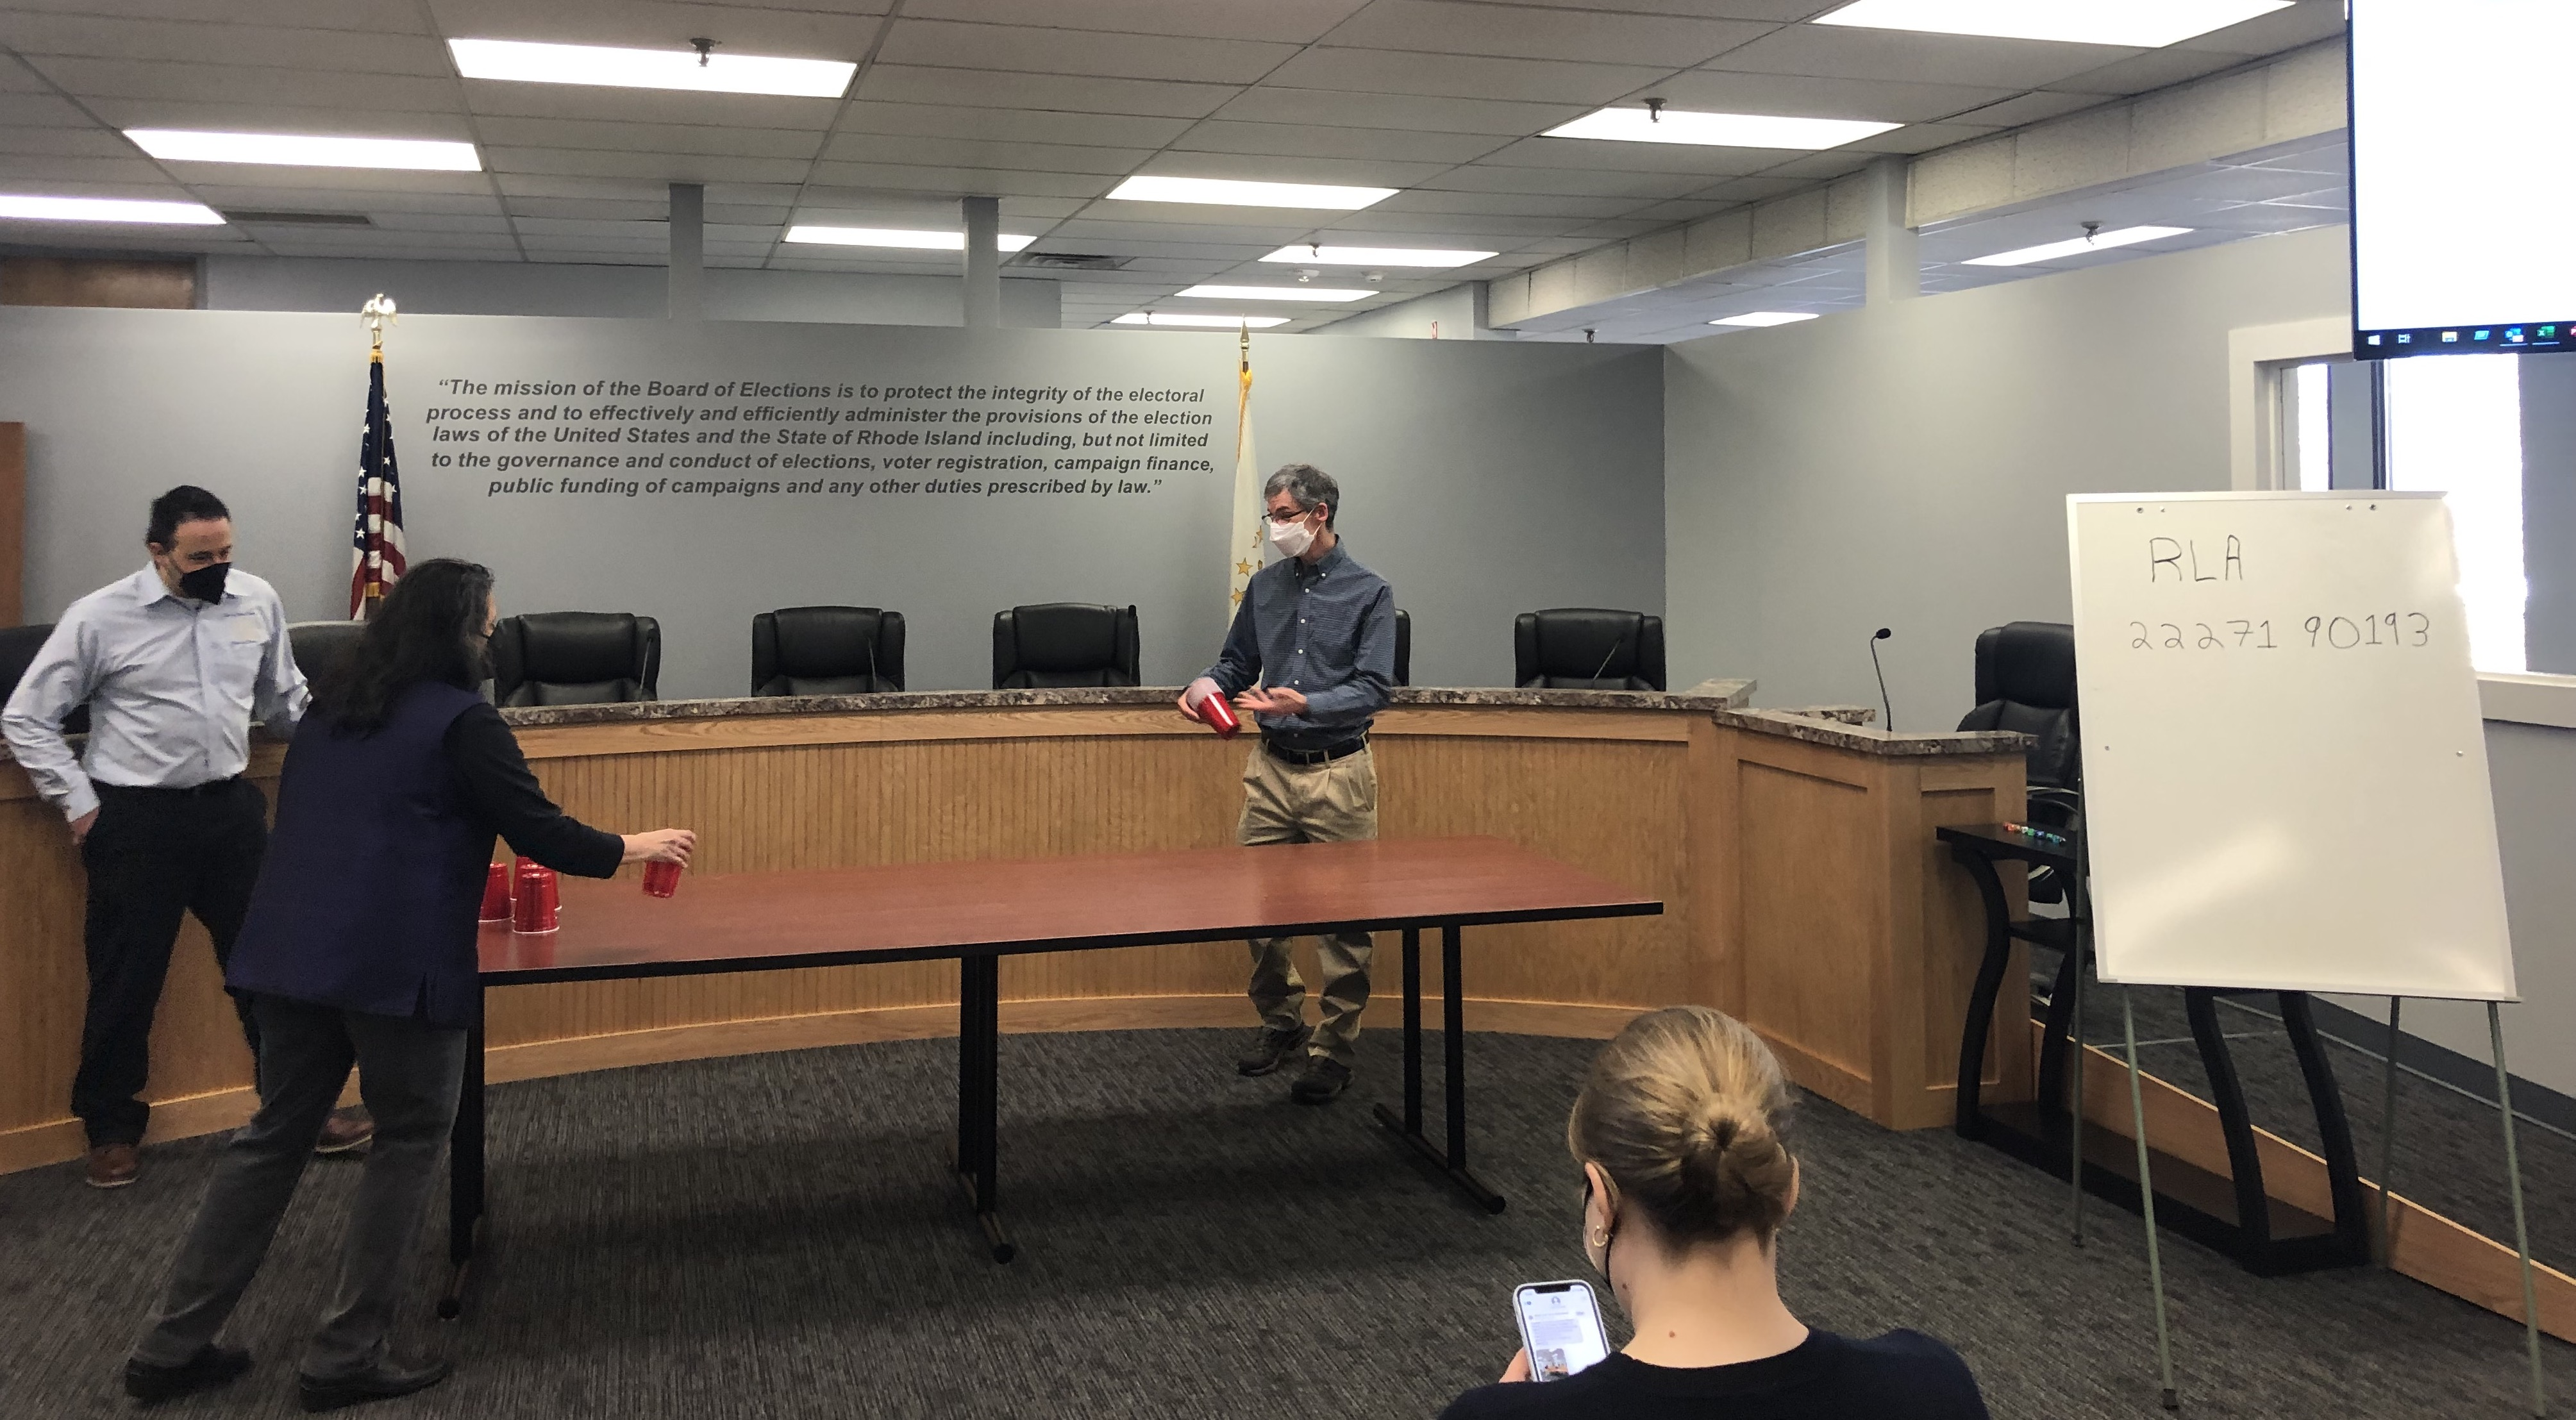
\includegraphics[width=1.0\textwidth]{dice.jpg}
\caption{
Professor Vora tosses her random-seed-generating 10-sided die, in a roll she dedicated to election officials everywhere.
The standing people from left to right are (1) Miguel Nunez, Rhode Island Deputy Director of Elections, 
(2) Professor Vora, and (3) Mark Lindeman, Verified Voting Director.
}
\end{figure}

\end{block}

\begin{block}{Simulations}

\emph{Need to fill in simulation results here. I am thinking (a) risk simulations as evidence that \Prov is an RLA, and (b) number of ballot results if I get them done quickly enough.}

Simulations are currently running to explore the risk, stopping probability, and number of ballots used by \Prov.

\end{block}



  \begin{block}{References}

    %\nocite{*}
    %\footnotesize{\bibliographystyle{plain}\bibliography{audits}}
    \bibliographystyle{splncs04}
    %\bibliographystyle{plain}
    \bibliography{audits}
    \emph{Having some latex trouble here, but should include r2b2, the recent simulations paper, bravo paper, athena paper, ...}

  \end{block}


\end{column}

\separatorcolumn

\end{columns}

\end{frame}

\end{document}

